\documentclass[a4paper,11pt]{ctexart}

\input{./Header.Tex}

% 部分使用说明
% \begin{lstlisting}[language={C}]
% 正式代码在此输入
% \end{lstlisting}

% \begin{codebox}
% 伪代码在此输入
% \end{codebox}

\begin{document}

\begin{titlepage}
\begin{center}

% 页面正中央插入的图片及哈尔滨工业大学英文全称
\includegraphics[width=0.8\textwidth]{./images/HIT.eps}\\[1cm]
\textsc{\LARGE Harbin Institute of Technology}\\[1.5cm]

% 标题
\hrulefill \\[0.4cm]
{ \huge \bfseries 电路分析报告}\\[0.4cm]
\hrulefill \\[1.5cm]

% 作者和其他信息
\begin{minipage}{0.4\textwidth}
\begin{flushleft} \large
% 左侧悬空
\end{flushleft}
\end{minipage}

% 右侧
\begin{minipage}{\textwidth}
\begin{flushright} \large
\emph{作者:}冯云龙\\
\emph{学号:}1160300202
\end{flushright}
\end{minipage}

\vfill
{\large \today}% 底部插入当日日期
\end{center}
\end{titlepage}

\part*{摘要}生活中有各种各样的电器设备,它们的电路设计往往非常精巧和实用,我们可以通过已有的电路基础知识分析一下它们的工作原理,了解它们为什么是这样工作的。
\paragraph{关键词:电路\ 电风扇\ 原理}

\tableofcontents            % 生成目录并隔开正文
\newpage

%\part*{正文}

\section{电风扇的类型}
\paragraph{按自动化程度分类}可分为普通电风扇和高档电风扇。
\paragraph{使用电源分类}可分为交流电风扇、直流电风扇和交直流电风扇。
\paragraph{电动机形式分类}可分为单相交流罩极式、单相交流电容式及交直流两用的串激式电风扇。
\paragraph{按结构特征及用途分类}可分为台扇、吊扇、落地扇、排气扇、转页扇等。
\begin{center}
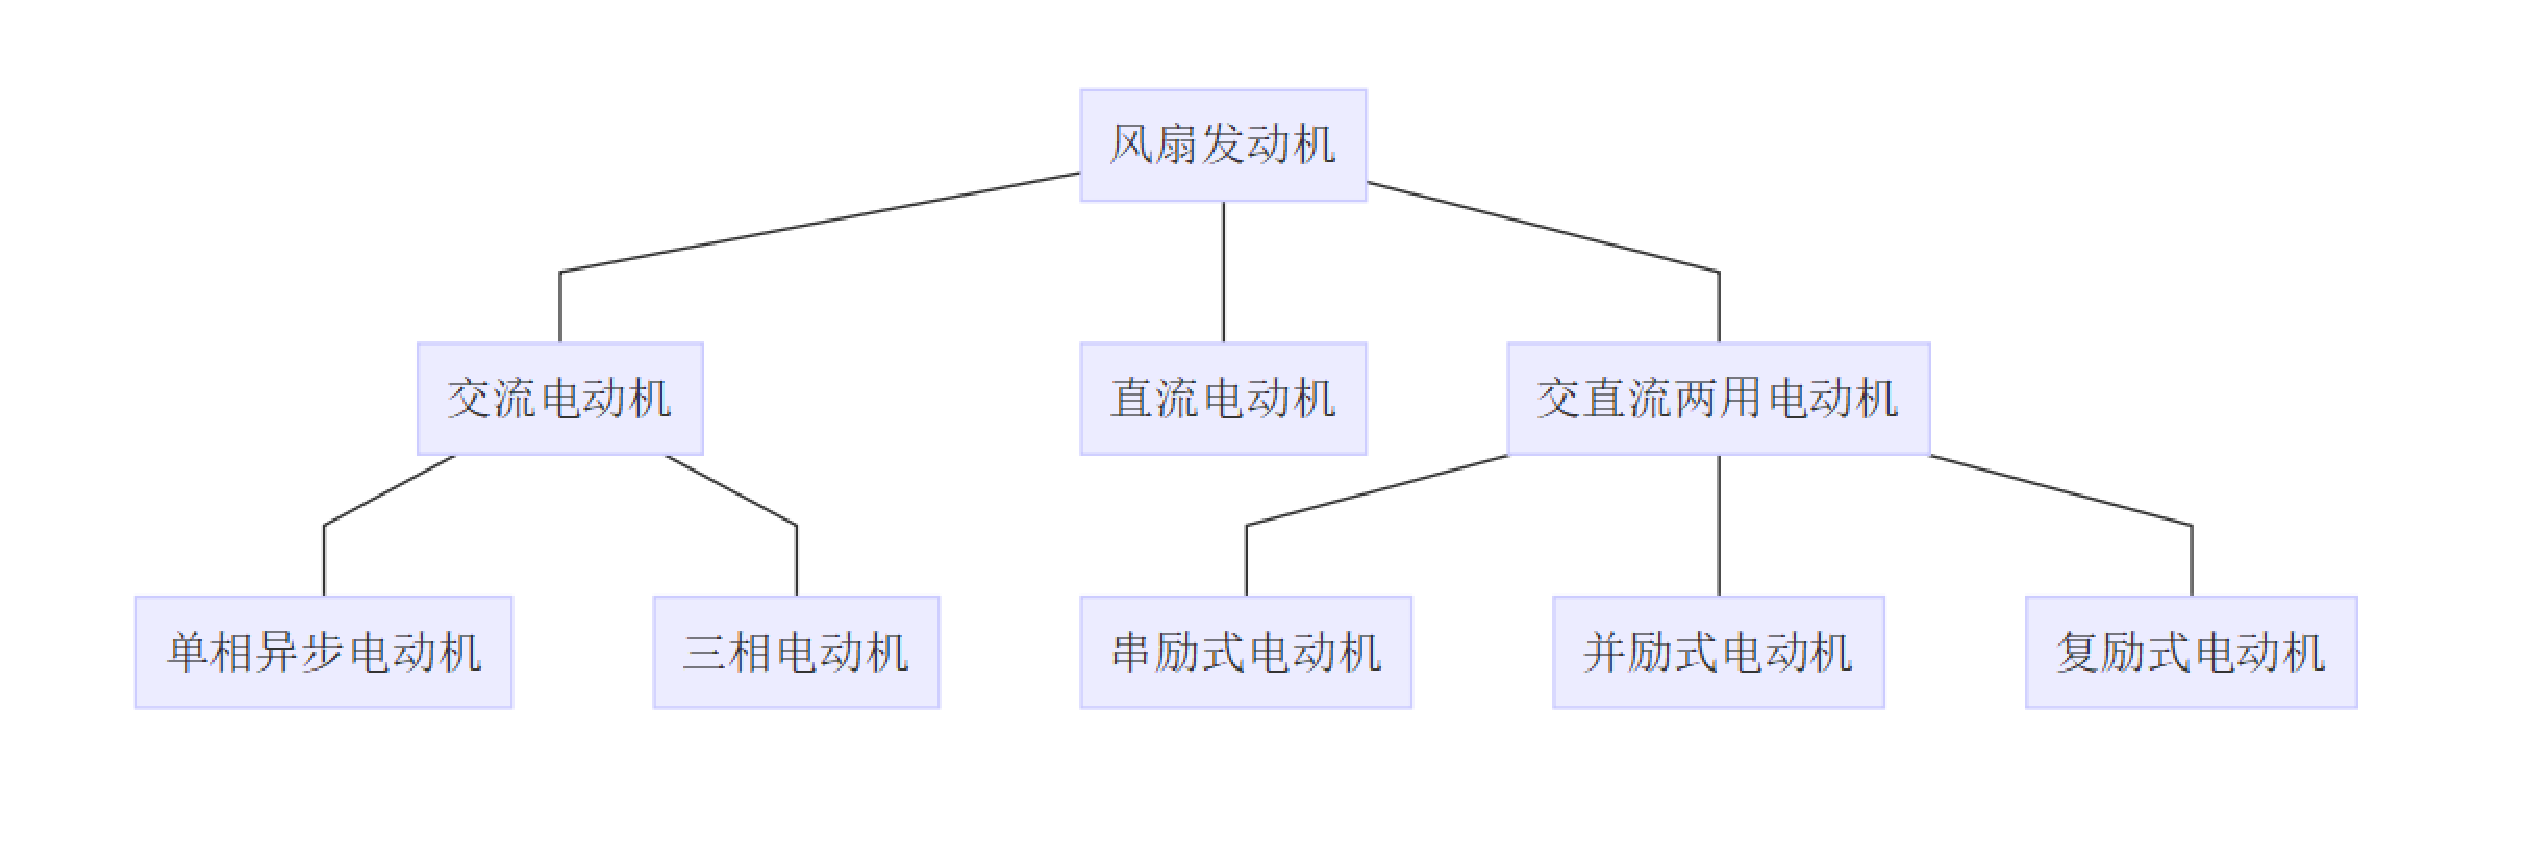
\includegraphics[width=0.8\textwidth]{./images/class.eps}
\end{center}


\section{电动机工作原理}
\subsection{单相异步交流电动机的工作原理}
单相异步交流电动机的工作绕组接通电源后,就会在气隙内产生一个大小相等、方向相反的脉振磁场,当该磁场切割转子导条后,将在导条中感应出相应的电势和电流,当转子电流与磁场作用时产生相应的电磁转矩。最终转矩等于零(即转子不转),必须借助起动绕组和电容器,来削弱其中一个方向的磁场,使在起动时气隙中能够形成一个旋转磁场。从而驱动转子顺着增强磁场的旋转方向转动。
\subsection{单相电容起动异步交流电动机}
电容起动电动机在副绕组串接一个离心开关和电容器与主绕组并接到单相电源上。电容的作用是使副绕组电流相位接近超前于主绕组电流相位90°电角度,有利于电动机起动。当转子的转速达到额定转速的75%左右时,由于离心力作用,离心开关被打开,副绕组支路开路,主绕组工作,维持电动机运行。
\subsection{单相电容转异步交流电动机}
电容运转电动机无论在启动或运转时,其副绕组与电容器串联并接到电源两端。这种运行方式,实质上是一台两相异步电动机,其两个绕组在空间相隔90°电角度,绕组中的电流在时间上也相差90°相角。定子绕组在气隙中产生的磁场接近圆形旋转磁场,使电动机的性能有较大的改善。这种电动机的功率因数、效率及过载能力都比普通单相异步交流电动机高。由于电动机在运行时需要的电容比启动时小,所以在电动机启动后,必须利用离心开关把多余的电容C1(起动电容)切除,而另一电容C2(运行电容)仍与副绕组接通。
\begin{center}
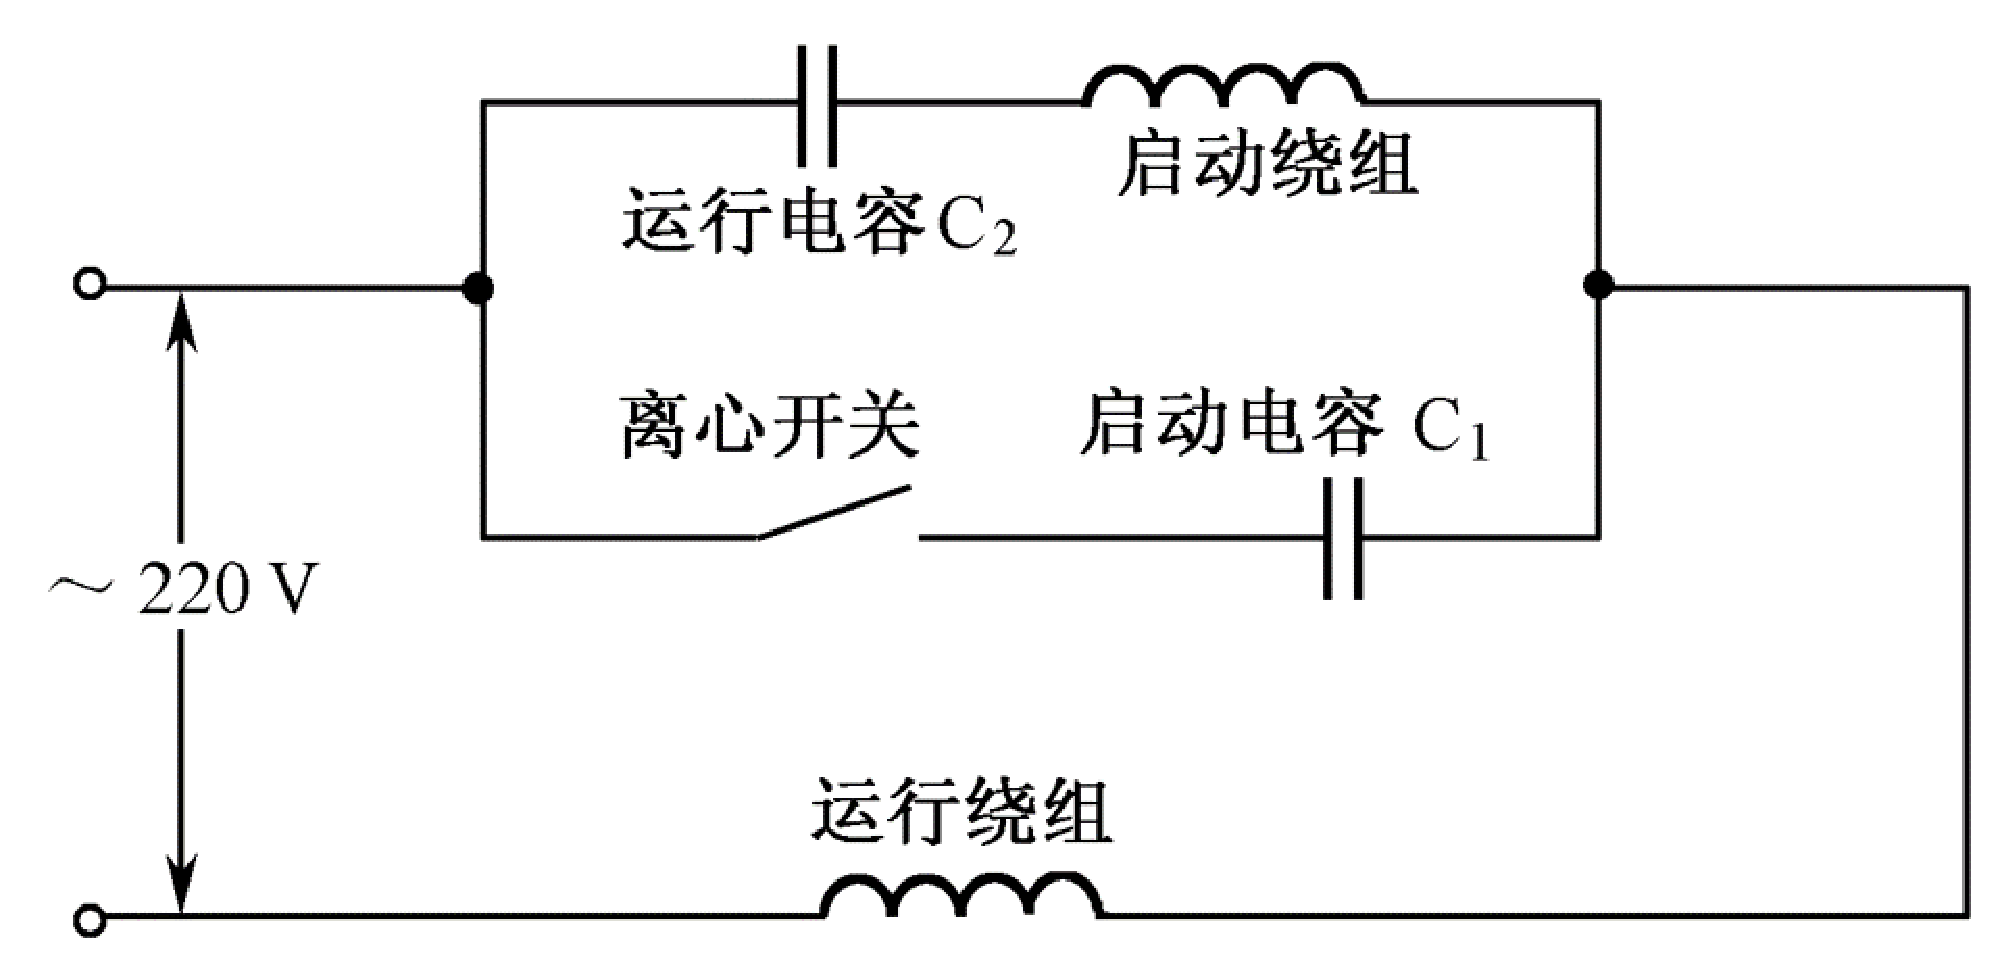
\includegraphics[width=0.8\textwidth]{./images/pic_1.eps}
\end{center}
\subsection{电容运转式电动机的优缺点}
\paragraph{优点}起动性能好、运转平稳、结构简单、效率高和噪音小。调速方便,在线圈中串电阻器或电抗器可以用来减速。
\paragraph{缺点}起动转距小,一般只有满载的50%~90%。

\section{电风扇的调速方法及原理}
\subsection{电抗器法}
在电路中串联电抗器,使电动机上的实际电压下降,电动机的转速也下降。 这种调速方法简单,运行可靠,但电动机运行效率不高。
当开关打在不同的档位时,串联在电风扇电路中的电抗器感抗XL大小就不同,所以风扇电路中的电流大小不同,风扇的转速就不同。
\begin{center}
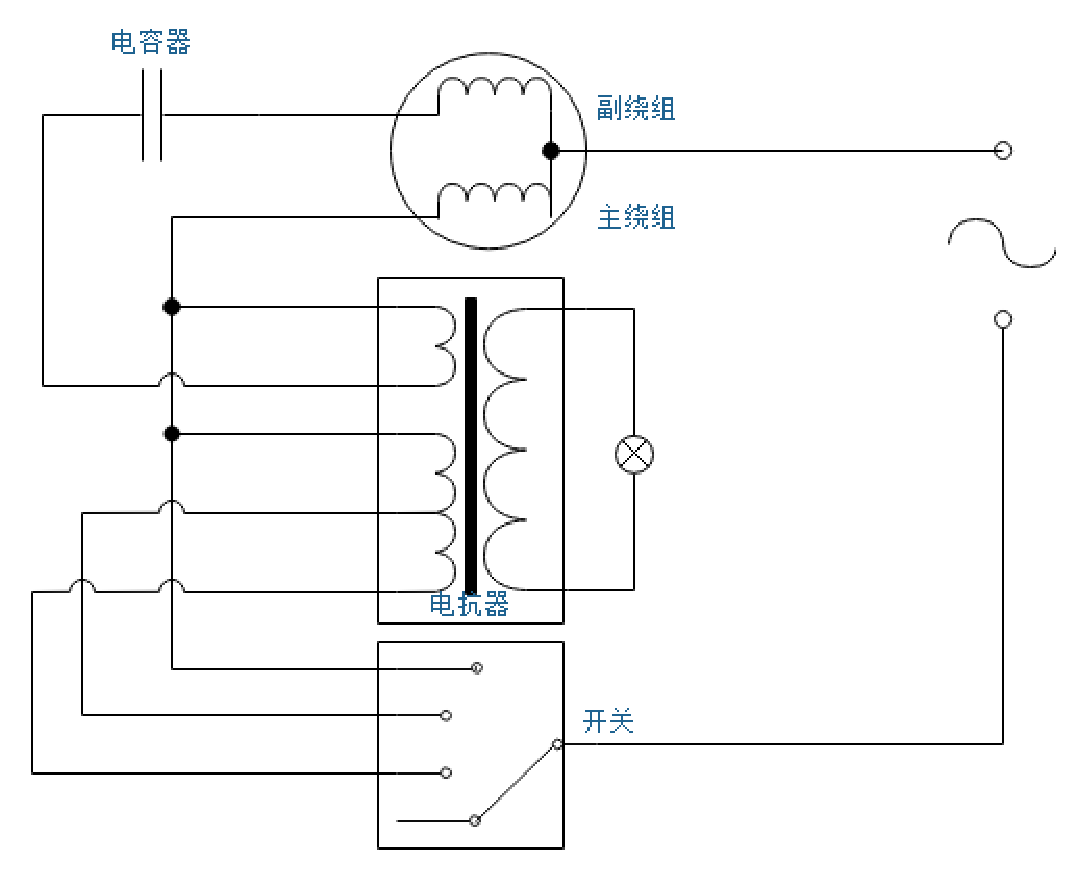
\includegraphics[width=0.7\linewidth]{./images/pic_2.eps}
\end{center}

\subsection{抽头法}
抽头调速是将电抗器和电动机结合在一起,在电动机定子铁心上嵌入一个调速绕组(或称中间绕组),在调速绕组上抽出几个头,接到调速开关。通过抽头转换,改变运转绕组与起动绕组之间的匝数比,从而改变磁场强度,调节电动机的转速。抽头法的特点是省去了电抗器,损耗小、重量轻,缺点是接线复杂,一般用于四极的电容式电动机。根据调速绕组与运转绕组和起动绕组的接线不同,常用的有L型接法和T型接法。
\subsubsection{L型抽头法}
L型调速可分为$L_I$型、$L_{II}$型、$L_{III}$型三种接线方式,如图所示。$L_I$型是主绕组(运转绕组)与调速绕组串联,它们是同相位,而它们与副绕组(起动绕组)在空间上相差90°。在调速绕组上抽两个头,可得高、中、低三挡。$L_I$型适用于较低电压(如110V)。$L_{II}$型是调速绕组与副绕组串联,它们与主绕组相差90°。$L_{II}$型适用于较高电压(如220V)。$L_{III}$型是调速绕组与主绕组同相位,调速时,调速绕组部分或全部与主绕组串联,而副绕组与电容器串联直接接在电源上,副绕组的端电压是不变的。
\begin{center}
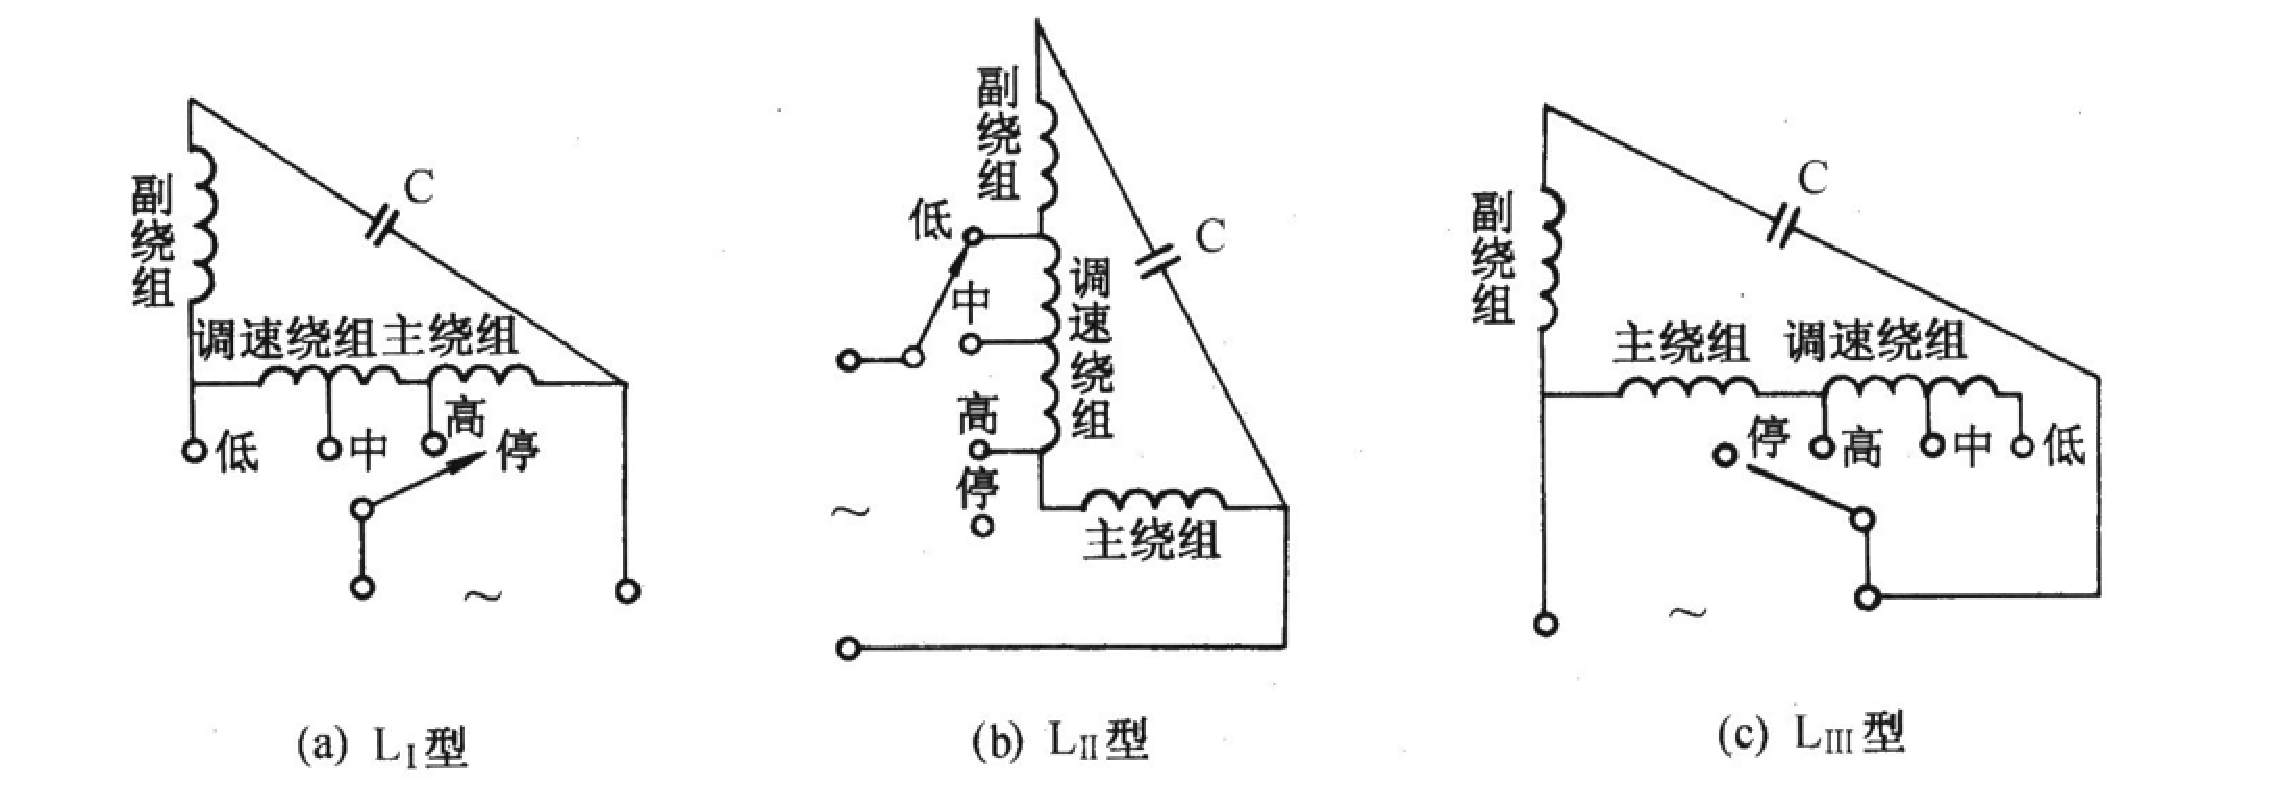
\includegraphics[width=0.8\linewidth]{./images/pic_3.eps}
\end{center}
\subsubsection{T型抽头法}
T型抽头调速是在原高速挡基础上外加一部分线圈,产生一定压降进行调速的,其作用与电抗器相似。或在原高速挡主、副绕组基础上,通过改变抽头位置,减少主绕组或副绕组的匝数调速。
T型抽头调速可分为$T_I$型和$T_{II}$型两种,如图所示。在$T_I$型接法中,调速绕组接在主副绕组之外,调速绕组在空间上与主绕组同相位。在$T_{II}$型接法中,调速绕组与副绕组在空间上同相位。由于$T_I$型比$T_{II}$型接法简单,实际应用中多采用$T_I$型接法,这种方法适用于较高电压( 220V),而且能提高电动机的效率,增大起动转矩,有利于低速起动。
\begin{center}
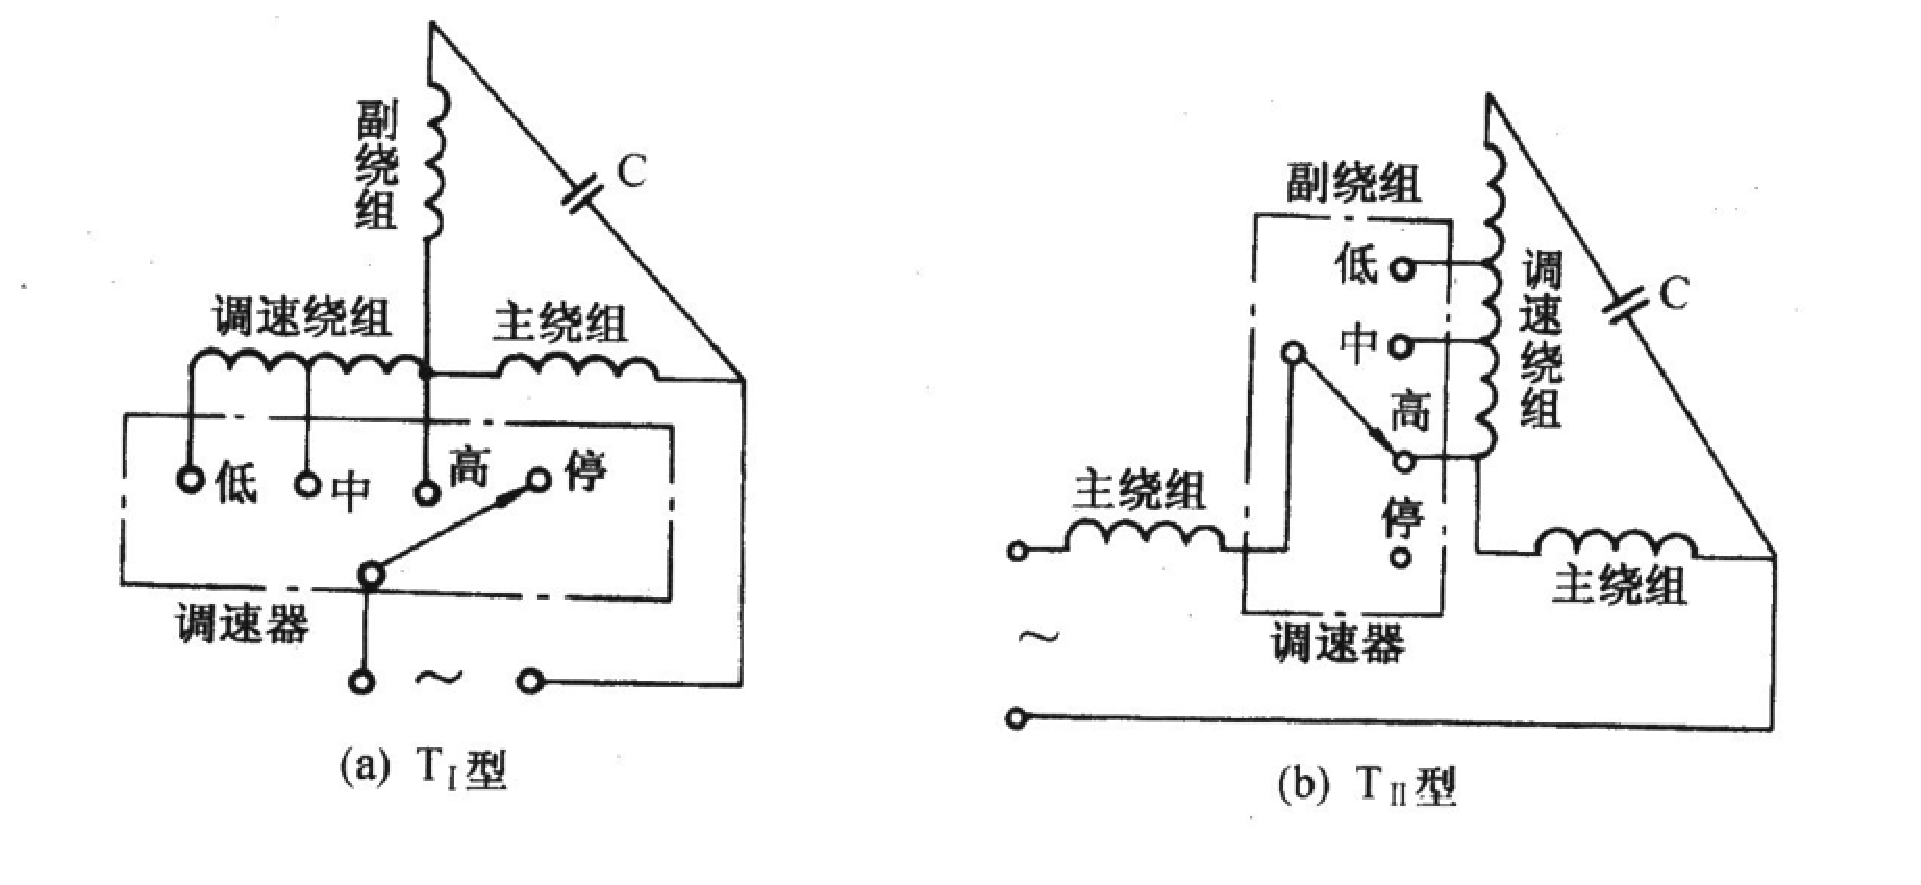
\includegraphics[width=0.8\linewidth]{./images/pic_4.eps}
\end{center}

\section{总结}
尽管只是普普通通的电风扇,其设计之精巧令人惊讶,这里仅仅分析了调速部分的电路,关于自然风、红外遥控、定时等电路还更加巧妙。由于相关的知识储备不足,这里并不能将其全部分析,实在是有些遗憾。

%\newpage
%\appendix
%\part{附录}


\end{document} 